\documentclass[10pt]{beamer}

%Paquetes
\usepackage[utf8]{inputenc}
\usepackage[T1]{fontenc}
%\usepackage{babel}

\usepackage{svg}
\usepackage{adjustbox}
\usepackage{textcomp}
\usepackage{csquotes}
\usepackage{amsmath}
\usepackage{multirow}
\usepackage[autocite=footnote,backend=biber, maxnames=3]{biblatex}
\usepackage{tabularx}
\usepackage{epstopdf}
%Bibliografía
\addbibresource{refs.bib}
%Tema
\usetheme[compress]{Berlin}

\makeatletter
\setbeamertemplate{footline}
{
  \leavevmode%
  \hbox{%
  \begin{beamercolorbox}[wd=.333333\paperwidth,ht=2.25ex,dp=1ex,center]{author in head/foot}%
    \usebeamerfont{author in head/foot}\insertshortauthor
  \end{beamercolorbox}%
  \begin{beamercolorbox}[wd=.333333\paperwidth,ht=2.25ex,dp=1ex,center]{title in head/foot}%
    \usebeamerfont{title in head/foot}\insertshorttitle
  \end{beamercolorbox}%
  \begin{beamercolorbox}[wd=.333333\paperwidth,ht=2.25ex,dp=1ex,right]{date in head/foot}%
    \usebeamerfont{date in head/foot}\insertshortdate{}\hspace*{2em}
  \end{beamercolorbox}}%
  \vskip0pt%
}
\makeatother

%Título:
\title{Identification of Racial and Sexist Stereotypes in Spanish}
\subtitle{A Learning with Disagreements Approach \\ \small{In: Procesamiento del Lenguaje Natural (SEPLN), num. 74 (accepted)}}
\author[Elias Urios Alacreu]{Elias Urios Alacreu \inst{1} \and Paolo Rosso \inst{1,2}}
\institute[shortinst]{\inst{1} PRHLT Research Center, Universitat Politècnica de València \\ \inst{2} ValgrAI Valencian Graduate School and Research Network of Artificial Intelligence}
% Preamble
\setbeamertemplate{itemize subitem}[circle]
\setbeamertemplate{itemize subsubitem}[triangle]
\AtBeginSection[]
{
  \begin{frame}
    \frametitle{Index}
    \tableofcontents[currentsection]
  \end{frame}
}

\titlegraphic{%
  \makebox[\textwidth]{%  <-- The box with full width
    \centering % Center the content within the box
    \adjustbox{valign=c, width=1.5cm}{\includesvg{images/marca_UPV_secundaria_negro.svg}}%
    \hspace{0.25cm} % Or your desired horizontal space
    \adjustbox{valign=c, width=3cm}{
\includegraphics{images/logoprhlt_mobil.png}}%
  }%
}

\renewcommand\footfullcite[1]{%
\begingroup
\renewcommand\thefootnote{}\footnote{\fullcite{#1}}%
\addtocounter{footnote}{-1}%
\endgroup
}




\renewcommand{\footnotesize}{\scriptsize}

\begin{document}

%Índice general
\frame{\titlepage}
\begin{frame}
\frametitle{Index}
\tableofcontents
\end{frame}


%Introducción
\section{Introduction}
\begin{frame}{Introduction}
    % Slide 1: Introduction to HS
        \begin{columns}
        \column{0.65\textwidth}
            \begin{itemize}
                \item HS is an acknowledged phenomenon:
                \begin{itemize}
                    \item Social media platforms
                    \item Increasingly sheer volume of content
                    \item Change of policies
                \end{itemize}
                \item Targets:
                \begin{itemize}
                    \item LGTBQ+
                    \item Black community
                    \item \textbf{Women}
                    \item \textbf{Immigrants}
                \end{itemize} 
                \item Hate speech incites violence and intolerance
                \item Transformers for addressing HS
            \end{itemize}
        \column{0.35\textwidth}
                
\includegraphics[width=\textwidth]{images/x_hate.PNG}
                \vfill
                
\includegraphics[width=\textwidth]{images/meta_new_policy.PNG}
                \vfill
                
\includegraphics[width=\textwidth]{images/homofobia.PNG}
        \end{columns}
        \footfullcite{oberaxe}
\end{frame}

\begin{frame}{Challenges of addressing HS}
    \begin{columns}
        \column{0.5\textwidth}
        \begin{itemize}
            \item Lack of a universal definition
        \item Intersection with various fields/areas
        \item Lack of resources outside of English
        \item Forms of expression:
            \begin{itemize}
        \item Aggressive: threats, violence
        \item Non-aggressive: humor, irony, \textbf{stereotypes}
            \end{itemize}
        \item Type of content:
            \begin{itemize}
            \item Text (mostly addressed)
            \item Multimodal (images, videos, \textbf{memes})
            \end{itemize}
        \item \textbf{Subjectivity}
        \end{itemize}
        \column{0.6\textwidth}
        \begin{quote}
            \textit{[...] the lack of definitions in scholarship translates to uncertain definitions
            in law and social science research, and even more uncertain application of
            principles in on-line spaces}
        \end{quote}
        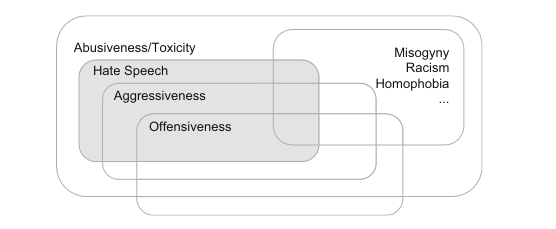
\includegraphics[width=\textwidth]{images/marco-hate.png}
\end{columns}
\footfullcite{sellars2016defining,Poletto2021}
\end{frame}

\begin{frame}{Deep learning and HS}

    \only<1->{\begin{alertblock}{DL limitations in HS}
        It is clear that automated methods, especially those based on DL, are necessary to address HS. However, the usage of black box methods involves ethical concerns.
    \end{alertblock}
    }
    \only<2->{
    \begin{block}{Addressing the limitations}
        What if we trained our models to see beyond black and white? What if we had more debiased datasets? What if we paid attention to all opinions?
    \end{block}
    }
\end{frame}

\begin{frame}{Research Questions}
    \begin{itemize}
        \item \textbf{RQ1}: How does the LeWiDi paradigm influence a classifier performance for detecting racial stereotypes in online comments and discussion forums?
        \item \textbf{RQ2}: How does the LeWiDi paradigm influence a classifier performance for detecting sexist stereotypes in memes?
        \item Shared tasks:
        \begin{itemize}
            \item \textbf{DETEST-Dis}: \textit{DETEction and classification of racial STereotypes in Spanish - Learning with Disagreement}
            \item \textbf{EXIST}: \textit{sEXism Identification in Social neTworks}
        \end{itemize} 
    \end{itemize}
\end{frame}

%leWiDi
\section{LeWiDi}
\begin{frame}{LeWiDi: Why?}
\begin{itemize}
    \item Supervised tasks require annotated data
    \item Data annotation is a time-consuming and expensive process
    \item Assumption: existence of a single, objective truth
    \item Reality: disagreements often arise
    \item Reasons
    \begin{itemize}
        \item Mistakes/slips from the annotators
        \item Poor annotation schemes
        \item \textbf{Subjectivity}
        \item ...
    \end{itemize}
    \item Why would we ignore the minority over the majority?
\end{itemize}
\footfullcite{lewidi_survey}
\end{frame}
%Include examples

\begin{frame}{LeWiDi: Beyond black and white}
\begin{itemize}
    \item Aggregate annotations into a gold truth (\textbf{hard label})
    \begin{itemize}
        \item Majority voting (traditional approach)
        \item Probabilistic methods: MACE 
    \end{itemize}
    \item Ignore ``difficult`` labels by using disagreement
    \item Aggregate annotations into a probability distribution (\textbf{soft label})
    \begin{itemize}
        \item Probability or softmax
        \item Soft loss function (\textbf{CE}, KL or MSE)
    \end{itemize}
    \item Combine information from \textbf{hard} and \textbf{soft} labels
    \item Perspectivist: work directly with non-aggregated annotations
\end{itemize}
\footfullcite{lewidi_survey,Frenda2024}
 \end{frame}

\begin{frame}{LeWiDi: Evaluation}
    \begin{itemize}
        \item Hard evaluation: Traditional evaluation using hard labels
        \begin{itemize}
            \item Common metrics: F1-Score, Accuracy, Information Contrast Metric (ICM)
            \item Traditional approach usually works the best
            \item Soft loss can be better under certain conditions
        \end{itemize}
        \item Soft evaluation: How well does the model generalize
        \begin{itemize}
            \item Common metrics: CE, JSD, KL, ICM Soft
            \item Soft loss works the best
        \end{itemize}
    \end{itemize}
\end{frame}

%SOTA
%\section{Estado del Arte}
%TEXTO
\begin{frame}{Clasificaci\'on con modelos de texto}

   \begin{itemize}
    \item \textit{Transformer encoder} preentrenado: \textit{Robustly optimized BERT approach} (RoBERTa) \footfullcite{liu2019robertarobustlyoptimizedbert}
    \item \textit{Fine-tuning} junto con \textit{token} especial para la  clasificaci\'on ([CLS])
    \item Modelo monoling\"ue preferible a uno multiling\"ue
    \item Tareas destacables: EXIST, DETESTS, AMI (\textit{Automatic Misogyny Identification})
\end{itemize}
\end{frame}

%MULTIMODAL
\begin{frame}{Clasificaci\'on con modelos multimodales}
    \begin{itemize}
        \item \textit{Early Fusion}: Fusionar modalides de arquitecturas unimodales a trav\'es de alg\'un mecansimo
        \item Modelos preentrenados orientados a alinear texto e imagen:
        \begin{itemize}
            \item CLIP (\textit{Contrastive Language-Image Pre-Training})
            \item VisualBERT
            \item FLAVA (\textit{Foundation Language And Vision Alignment})
        \end{itemize}
        \item Texto $\gg$ Imagen  para los memes 
        \item Tareas destacables: MAMI (Multimedia Automatic Misogyny Identification), Hateful Memes Challenge
    \end{itemize}
\footfullcite{aggarwal-etal-2024-text}
\end{frame}

%LeWiDi
\begin{frame}{LeWiDi}
\begin{itemize}
    \item Enfoque cl\'asico: 
    \begin{itemize}
        \item Asumir la existencia de una verdad absoluta
        \item Votaci\'on mayoritaria o m\'etodos probabil\'isticos
        \item Mejor para la evaluaci\'on \textit{hard}
    \end{itemize}
    \item Enfoque perspectivista:
    \begin{itemize}
        \item Modelar las anotaciones individuales
        \item \textit{Ensemble}, \textit{multi-label} y \textbf{\textit{multi-task}}
    \end{itemize}
    \item Enfoque \textit{soft loss}: 
    \begin{itemize}
        \item Agregar las anotaciones en una distribuci\'on: \textit{Softmax} o emp\'irica 
        \item $\mathcal{L}$: \textbf{\textit{Cross Entropy}}, Kullback-Leibler y \textit{Minimum Square Error}
        \item Enfoque que m\'as generaliza
    \end{itemize}
\end{itemize}
\footfullcite{lewidi_survey}
\end{frame}

\begin{frame}{M\'etricas}
    \begin{columns}[T]
        \column{0.5\textwidth}
        \centering
        \textbf{Evaluaci\'on \textit{hard}}
        \vspace{0.25cm}
        \begin{itemize}
            \item $F_1$ \textit{score}:
            $$ F_1 =  2\frac{P \cdot R}{P + R} $$
            \item \textit{Information Contrast Metric} (ICM) 
            \begin{align*}
                ICM(A, B) &= \alpha_1IC(A) + \alpha_2IC(B) \\
                          &- \beta IC(A \cup B) \\
                IC(A) &= -\log_2P(A)
            \end{align*}
        \end{itemize}
        
        \column{0.5\textwidth}
        \centering
        \textbf{Evaluaci\'on \textit{soft}}
        \vspace{0.25cm}
        \begin{itemize}
            \item \textit{Cross Entropy}
            \begin{align*}
                CE(p, q) = - \sum_{x \in \mathcal{X}} p(x) \log_2q(x)
            \end{align*}
            \item \textit{ICM Soft}: ICM adaptada para distribuciones de probabilidad
            $$
            IC(\{c_i, v_i\}) = -log_2(P(\mathcal{I}_c \geq v))
            $$
        \end{itemize}
    
    \end{columns}
    \footfullcite{amigo-delgado-2022-evaluating}
\end{frame}
%DETEST-DIS new
\section{DETESTS-Dis}

\begin{frame}{Task descriptions}
    \only<1>{
    \begin{columns}
    \column{0.5\textwidth}
    \centering
    \begin{itemize}
        \item Second edition of DETESTS
        \item Stereotype detection on text
        \item Framed within LeWiDi: 
        \begin{itemize}
            \item Aggregated annotations: majority voting and softmax
            \item Non-aggregated annotations
        \end{itemize}
        \item Two tasks:
            \begin{itemize}
                \item \textbf{Stereotype detection}: binary classification task 
                \item \textbf{Stereotype implicitness detection}: novel hierarchy classification task 
            \end{itemize}
        \footfullcite{detests_dis_2024}
    \end{itemize}

    \column{0.5\textwidth}
    \centering
    \includesvg[width=0.8\textwidth]{images/DETEST-tareas.svg}
        \begin{table}[]
            \small
            \centering
            \resizebox{\textwidth}{!}{%
            \begin{tabular}{|c|c|c|}
            \hline
            Task       & Hard evaluation & Soft evaluation \\ \hline
            Stereotype & F1              & CE              \\ \hline
            Implicit   & ICM             & ICM Soft        \\ \hline
            \end{tabular}
            }
        \end{table}
    \end{columns}
    }
    \only<2>{
        \begin{table}[]
            \centering
            \begin{tabularx}{\textwidth}{|X|c|c|}
            \hline
            \textbf{Text} & \textbf{Stereotype} & \textbf{Implicitness} \\ \hline
            The solution is to develop a critical and esceptical thinking. & X & - \\ \hline
            Like it or not, one thing is clear: if there were no muslims in Europe, this wouldn't happen. & \checkmark & X \\ \hline
            Yesterday I was at the tax office, all Spaniards, in the afternoon I went to the health center, half of them Spaniards. & \checkmark & \checkmark \\ \hline
            \end{tabularx}
        \end{table}
    }
\end{frame}

\begin{frame}{Dataset}
   \only<1>{
    \begin{itemize}
        \item Comment threads from news articles
        \item Annotated by 3 expert annotators (2 linguistics and 1 researcher)
        \item Two corpora
        \item DETEST corpora:
        \begin{itemize}
            \item Corpus from the first edition
            \item Threads from online news forums
            \item Annotations are provided on a sentence level
        \end{itemize} 
        \item StereoHOAX corpora:
        \begin{itemize}
            \item New corpora for this edition
            \item Threads from Twitter
            \item Annotations are provided on a tweet level
        \end{itemize}
        \item Different levels of context:
        \begin{itemize}
            \item \textbf{Level 1}: Previous sentence (DETEST)
            \item \textbf{Level 2}: Previous tweet/comment
            \item \textbf{Level 3}: First tweet/comment
            \item \textbf{Level 4}: News text
        \end{itemize}
    \end{itemize}
   }
   
    \only<2>{
        \begin{columns}[T]
        \column{0.5\textwidth}
        \centering
        Stereotype identification
        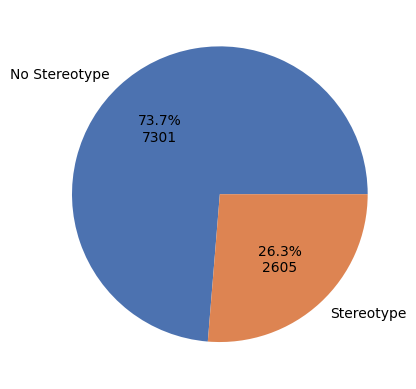
\includegraphics[width=\textwidth]{images/detest_hard_labels.png}

        \column{0.5\textwidth}
        Implicitness detection
        \centering
        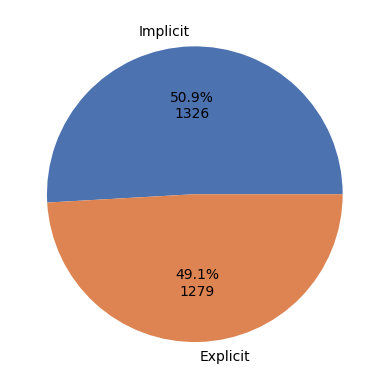
\includegraphics[width=\textwidth]{images/detest_soft_labels.png}
        \end{columns}
    }

\end{frame}

\begin{frame}{System proposals}
    \only<1> {
    \begin{columns}
    \column{0.6\textwidth}
    \begin{itemize}
        \item RoBERTa model as text encoder.
        \item \textbf{Hard label} approach
        \begin{itemize}
            \item Classic approach (comparison purposes)
            \item $\mathcal{L}(\hat{y}, y) = \text{BCE}(\hat{y}, y)$
        \end{itemize}
        \item \textbf{Soft label} approach
        \begin{itemize}
            \item Train by soft label probablity distribution
            \item $\mathcal{L}(\hat{y}, y) = \text{CE}(\hat{y}, y)$
        \end{itemize}
        \item \textbf{Perspectivist} approach
        \begin{itemize}
            \item \textbf{Multi-task proposal}: three classification heads with one output neuron each
            \item $\mathcal{L}(\hat{y}, y) = \sum_{a=1}^{3} \text{CE}(\hat{y_a}, y_a)$
            \item Aggregate outputs for predictions (majority voting and softmax)
        \end{itemize}
    \end{itemize}
    
    \column{0.4\textwidth}
    \centering
    \includesvg[width=4.5cm]{images/DETESTS-dis_presentacion.svg}
    \end{columns}
    }

    \only<2> {
    \begin{columns}
    \column{0.6\textwidth}
    \begin{itemize}
        \item Layer-Wise Learning Rate fine-tuning
        \begin{itemize}
            \item Deeper encoder layers recieve larger updates, shallowers receive smaller ones
            \item $\eta = \{1e-5, 2e-5, 5e-5, 1e-4\}$
            \item $\xi = \{1'0, 0'97, 0'95, 0'90\}$
        \end{itemize}
        \item Context inclusion:
        \begin{itemize}
            \item Append context via [SEP] token
            \item \textbf{DETEST} samples $\rightarrow$ Previous sentence
            \item \textbf{StereoHOAX} samples $\rightarrow$ First tweet
        \end{itemize}
        \item Back-translation on minority class (ES $\rightarrow$ EN $\rightarrow$ ES)
    \end{itemize}

    \column{0.4\textwidth}
    \centering
    \includesvg[width=4.5cm]{images/DETESTS-dis_presentacion.svg}
    \end{columns}
    }
\end{frame}


\begin{frame}{Stereotype detection: train}
    \only<1>{
    \begin{table}[H]
        \centering
        \resizebox{\textwidth}{!}{
        \begin{tabular}{c|cc|c|c}
                     & \multicolumn{2}{c|}{Hiperparámetros} & Hard Evaluation     & Soft evaluation     \\ \hline
        Architecture & \multicolumn{1}{c|}{$\xi$}  & $\eta$ & F1-Stereotype  $\uparrow$     & \textit{Cross Entropy} $\downarrow$                 \\ \hline
        \textit{Hard label}   & \multicolumn{1}{c|}{1.0}    & 1e-5   & 0.7380 $\pm$ 0.0222 & \textbf{0.6260 $\pm$ 0.0157} \\ \hline
        \textit{Hard label}   & \multicolumn{1}{c|}{0.95}   & 1e-5   & \textbf{0.7410 $\pm$ 0.0184} & 0.6308 $\pm$ 0.0125 \\ \hline \hline
        \textit{Soft label}   & \multicolumn{1}{c|}{1.0}    & 5e-5   & 0.7413 $\pm$ 0.0203 & 0.5979 $\pm$ 0.0250 \\ \hline
        \textit{Soft label}   & \multicolumn{1}{c|}{0.95}   & 5e-5   & \textbf{0.7488 $\pm$ 0.0175} & \textbf{0.5926 $\pm$ 0.0169} $\dagger$ \\ \hline \hline
        \textit{Multi-Task}   & \multicolumn{1}{c|}{1.0}    & 2e-5   & 0.7342 $\pm$ 0.0308 & 0.8191 $\pm$ 0.0411 \\ \hline
        \textit{Multi-Task}   & \multicolumn{1}{c|}{0.90}   & 2e-5   & \textbf{0.7519 $\pm$ 0.0163} $\dagger$ & \textbf{0.8094 $\pm$ 0.0350} \\ \hline
        \end{tabular}%
        }
        \caption{Comparison of normal fine-tuning with the best parameters found on hyperparameter search.}
        %\label{tab:detests_dis_hiper}
        \end{table}
    }
    \only<2>{
        \begin{columns}
            \column{0.55\textwidth}
            \centering
            Hard label approach
            \adjustbox{max width=\textwidth}{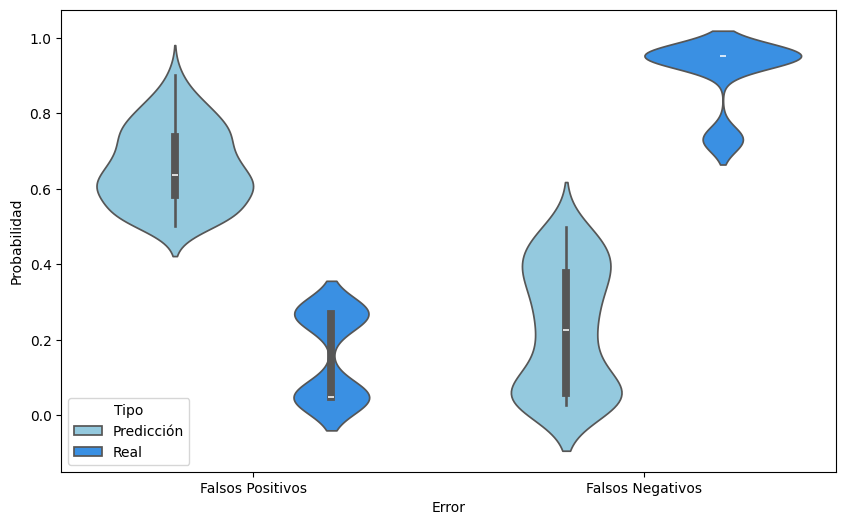
\includegraphics{images/violin_plot_hard.png}}
            
            \column{0.55\textwidth}
            \centering
            Soft label approach
            \adjustbox{max width=\textwidth}{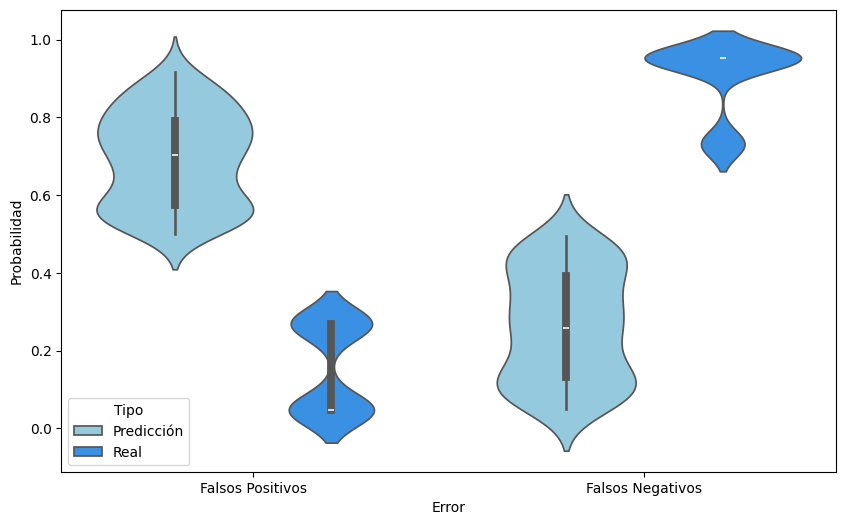
\includegraphics{images/violin_plot_soft.png}}
            
        \end{columns}
    }

    \only<3>{
        \centering
        Perspectivist approach
        \adjustbox{max width=\textwidth}{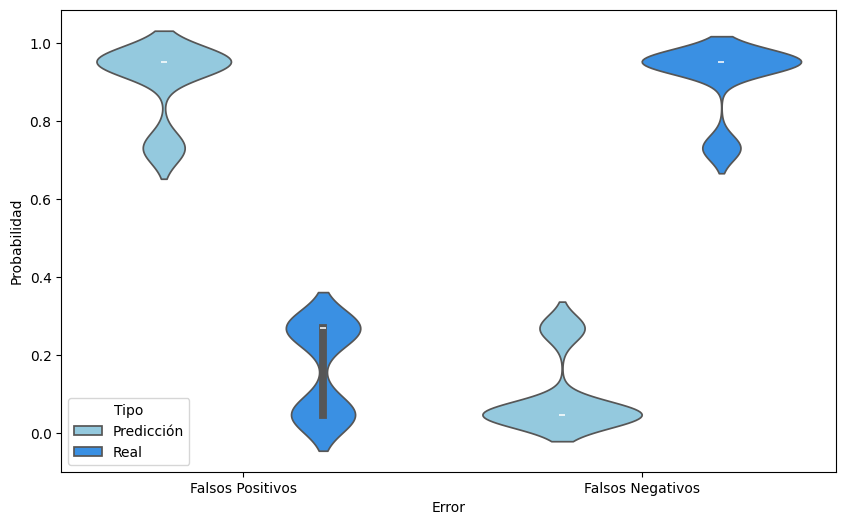
\includegraphics{images/violin_plot_annotators.png}}
    }
    \only<4>{
        \begin{table}[H]
            \centering
            \resizebox{\textwidth}{!}{
            \begin{tabular}{c|c|c}
                         & Hard Evaluation          & Soft evaluation     \\ \hline
            Architecture & F1-Stereotype $\uparrow$ & \textit{Cross Entropy} $\downarrow$     \\ \hline
            \textit{Hard label}   & 0.8713 $\pm$ 0.0081      & 0.6588 $\pm$ 0.0397 \\ \hline
            \textit{Soft label}   & 0.8980 $\pm$ 0.0046  $\dagger$    & 0.5177 $\pm$ 0.0076 $\dagger$ \\ \hline
            \textit{Multi-Task}   & 0.8829 $\pm$ 0.0084      & 0.6369 $\pm$ 0.0289 \\ \hline
            \end{tabular}
            }
            \caption{Back translation alongside context with each archicecture. $\dagger$ highlights the best results for each evaluation.}
            \label{tab:detests_dis_data_context_and_aug}
            \end{table}
    }

\end{frame}
\begin{frame}{Stereotype detection results: test}
    \begin{table}[hbt]
    \centering
    \resizebox{\textwidth}{!}{%
    \begin{tabular}{c|cc||cc|}
    \cline{2-5}
                                              & \multicolumn{2}{c||}{Hard evaluation}                       & \multicolumn{2}{c|}{Soft evaluation}                                      \\ \hline
    \multicolumn{1}{|c|}{Architecture}        & \multicolumn{1}{c|}{\# ranking/21} & F1 Score $\uparrow$ & \multicolumn{1}{c|}{\# ranking/8} & \textit{Cross Entropy} $\downarrow$ \\ \hline
    \multicolumn{1}{|c|}{\textit{Hard label}} & \multicolumn{1}{c|}{7}               & 0.653               & \multicolumn{1}{c|}{8}              & 1.409                               \\ \hline
    \multicolumn{1}{|c|}{\textit{Soft label}} & \multicolumn{1}{c|}{\textbf{4}}      & \textbf{0.691}      & \multicolumn{1}{c|}{\textbf{2}}     & \textbf{0.850}                      \\ \hline
    \multicolumn{1}{|c|}{\textit{Multi-task}} & \multicolumn{1}{c|}{5}               & 0.685               & \multicolumn{1}{c|}{7}              & 1.081                               \\ \hline \hline
    \multicolumn{1}{|c|}{Gold baseline}       & \multicolumn{1}{c|}{0}               & 1.000               & \multicolumn{1}{c|}{0}              & 0.255                               \\ \hline
    \multicolumn{1}{|c|}{Winners}           & \multicolumn{1}{c|}{1}               & 0.720               & \multicolumn{1}{c|}{1}              & 0.841                               \\ \hline
    \multicolumn{1}{|c|}{Baseline BETO}       & \multicolumn{1}{c|}{6}               & 0.663               & \multicolumn{1}{c|}{4}              & 0.893                               \\ \hline
    \end{tabular}%
    }
    \caption{DETEST-Dis stereotype detection official test results. Our best results are highlighted in bold for each evaluation.}
    \label{tab:t1_detests}
    \end{table}
    \footfullcite{detests_dis_2024}
\end{frame}



\begin{frame}{Implicitness detection results: train}
    \only<1>{
        \begin{table}[hbt]
            \centering
            \resizebox{\textwidth}{!}{
            \begin{tabular}{c|cc|cc}
                                              & \multicolumn{2}{c|}{Hard evaluation}                        & \multicolumn{2}{c}{Soft evaluation}                                 \\ \hline
            \multicolumn{1}{c|}{Arquitectura} & \multicolumn{1}{c|}{ICM $\uparrow$}   & ICM Norm $\uparrow$ & \multicolumn{1}{c|}{ICM Soft $\uparrow$} & ICM Soft Norm $\uparrow$ \\ \hline
            \multicolumn{1}{c|}{\textit{Hard label}}   & \multicolumn{1}{c|}{\textbf{0.0095 $\pm$ 0.0726}}  & \textbf{0.5049 $\pm$ 0.0533}     & \multicolumn{1}{c|}{0.4277 $\pm$ 0.1586}     & 0.5632 $\pm$ 0.0238          \\ \hline
            \multicolumn{1}{c|}{\textit{Soft label}}   & \multicolumn{1}{c|}{-0.0459 $\pm$ 0.0748} & 0.4644 $\pm$ 0.0568     & \multicolumn{1}{c|}{0.0870 $\pm$ 0.3862}     & 0.5129 $\pm$ 0.0568          \\ \hline
            \multicolumn{1}{c|}{\textit{Multi-task}}   & \multicolumn{1}{c|}{-0.0498 $\pm$ 0.1230} & 0.4649 $\pm$ 0.0891     & \multicolumn{1}{c|}{\textbf{0.4981 $\pm$ 0.3719}}     & \textbf{0.5726 $\pm$ 0.0543}         
            \end{tabular}%
            }
            \caption{Train results for the implicitness detection task of DETEST-Dis. Our best results are highlighted in bold for each evaluation.}
            \end{table}
    }
    \only<2>{
        \begin{table}[hbt]
            \centering
            \begin{tabular}{c|c}
            Architecture & \textit{Cross Entropy} $\downarrow$          \\ \hline
            \textit{Hard label}  & 0.6639 ± 0.0208          \\ \hline
            \textit{Soft label}   & \textbf{0.6282 ± 0.0147} \\ \hline
            \textit{Multi-task}   & 0.8567 ± 0.0902         
            \end{tabular}%
            \caption{Cross-entropy training results for the DETEST-Dis implicitness detection task. Our best results are highlighted in bold.}
            \label{tab:results_detests_ce_t2}
        \end{table}
    }
\end{frame}


\begin{frame}{Implicitness detection results: test}
\begin{table}[]
    \centering
    \resizebox{\textwidth}{!}{%
    \begin{tabular}{c|ccc||ccc|}
    \cline{2-7}
                                              & \multicolumn{3}{c||}{Hard evaluation}                                                             & \multicolumn{3}{c|}{Soft evaluation}                                                                      \\ \hline
    \multicolumn{1}{|c|}{Architecture}        & \multicolumn{1}{c|}{\# ranking/14} & \multicolumn{1}{c|}{ICM $\uparrow$} & ICM Norm $\uparrow$ & \multicolumn{1}{c|}{\# ranking/6} & \multicolumn{1}{c|}{ICM Soft $\uparrow$} & ICM Soft Norm $\uparrow$ \\ \hline
    \multicolumn{1}{|c|}{\textit{Hard label}} & \multicolumn{1}{c|}{4}               & \multicolumn{1}{c|}{0.045}          & 0.516               & \multicolumn{1}{c|}{2}              & \multicolumn{1}{c|}{-0.917}              & 0.401                    \\ \hline
    \multicolumn{1}{|c|}{\textit{Soft label}} & \multicolumn{1}{c|}{\textbf{2}}      & \multicolumn{1}{c|}{\textbf{0.065}} & \textbf{0.524}      & \multicolumn{1}{c|}{3}              & \multicolumn{1}{c|}{-0.969}              & 0.396                    \\ \hline
    \multicolumn{1}{|c|}{\textit{Multi-task}} & \multicolumn{1}{c|}{3}               & \multicolumn{1}{c|}{0.061}          & 0.522               & \multicolumn{1}{c|}{\textbf{1}}     & \multicolumn{1}{c|}{\textbf{-0.900}}     & \textbf{0.403}           \\ \hline \hline
    \multicolumn{1}{|c|}{Gold baseline}       & \multicolumn{1}{c|}{0}               & \multicolumn{1}{c|}{1.380}          & 1.000               & \multicolumn{1}{c|}{0}              & \multicolumn{1}{c|}{4.651}               & 1.000                    \\ \hline
    \multicolumn{1}{|c|}{Baseline BETO}       & \multicolumn{1}{c|}{1}               & \multicolumn{1}{c|}{0.126}          & 0.546               & \multicolumn{1}{c|}{4}              & \multicolumn{1}{c|}{-1.124}              & 0.379                    \\ \hline
    \end{tabular}%
    }
    \caption{Test results for the implicitness detection task of DETEST-Dis. Our best results are highlighted in bold for each evaluation.}
    \label{tab:t2_detests}
    \end{table}
    \footfullcite{detests_dis_2024}
\end{frame}
%DETESTS
%\section{DETESTS-Dis}

\begin{frame}{Descripción de la tarea}
    \begin{columns}
        \column{0.5\textwidth}
            \begin{itemize}
                \item Segunda edición de DETESTS. Enmarcada dentro de LeWiDi.
                \item Dos tareas:
                    \begin{itemize}
                        \item \textbf{Detección de estereotipos}
                        \item \textbf{Categorización de estereotipos} en explícitos o implícitos 
                    \end{itemize}
                \item Dataset:
            \begin{itemize}
                \item Hilos de conversaciones (X y foros de noticias)
                \item Contexto proporcionado
                \item Etiquetas agregadas y sin agregar
                \item 3 anotadores (2 lingüistas y 1 investigador)
            \end{itemize}
    \end{itemize}
        \column{0.5\textwidth}
        \centering
        \includesvg[width=0.8\textwidth]{images/DETESTS-tareas.svg}
        % Please add the following required packages to your document preamble:
        % \usepackage{graphicx}
        \begin{table}[]
            \small
            \centering
            \resizebox{\textwidth}{!}{%
            \begin{tabular}{|p{3.5cm}|c|c|}
            \hline
            Texto                                                                                                                                                     & Estereotipo & Implícito  \\ \hline
            La solución es desarrollar el pensamiento crítico y escéptico.                                                                                            & X           & -          \\ \hline
            Guste o no guste la cosa está clara: si no hubiera moros en Europa esto no pasaría.                           & \checkmark  & X          \\ \hline
            Ayer estuve en hacienda tributando, todos españoles, por la tarde fui al centro de salud, españoles, la mitad. & \checkmark  & \checkmark \\ \hline
            \end{tabular}%
            }
            
            %\caption{}
            %\label{tab:my-table}
            \end{table}
    \end{columns}
\end{frame}

\begin{frame}{Análisis de los datos}
    \begin{columns}[T]
        \column{0.5\textwidth}
        \centering
        Identificación de estereotipos
        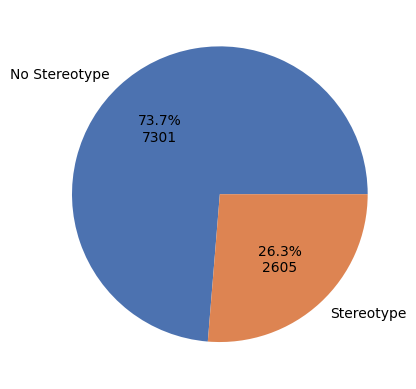
\includegraphics[width=\textwidth]{images/detest_hard_labels.png}

        \column{0.5\textwidth}
        Categorización de estereotipos
        \centering
        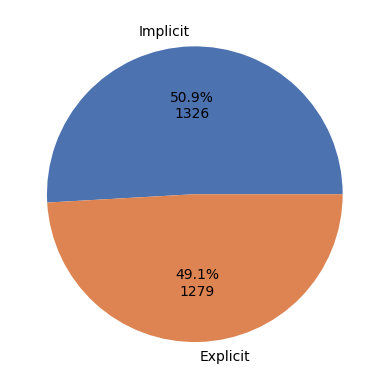
\includegraphics[width=\textwidth]{images/detest_soft_labels.png}
    \end{columns}

\end{frame}

\begin{frame}{Propuesta de sistema}
    \begin{columns}
    \column{0.6\textwidth}
    \begin{itemize}
        \item RoBERTa model as encoder. Our appro
        \item 
        \item Tres arquitecturas distintas
            \begin{itemize}
                \item \textit{Hard label}: Train by hard label, no disagreements considered
                \item \textit{Soft label approach}
                \item \textit{Multi-task}: Predecir cada anotación individualmente
            \end{itemize}

        \item \textit{Layer-Wise Learning Rate fine-tuning}
        \begin{itemize}
            \item Deeper layers are updated more aggresively than shallower layers
            \item $\eta = \{1e-5, 2e-5, 5e-5, 1e-4\}$
            \item $\xi = \{1'0, 0'97, 0'95, 0'90\}$
        \end{itemize}
        \item \textit{Back translation}
        \item Inclusión de Contexto
    \end{itemize}
    
    \column{0.4\textwidth}
    \centering
    \includesvg[width=4.5cm]{images/DETESTS-dis_presentacion.svg}
    \end{columns}
\end{frame}

\begin{frame}{Resultados detección de estereotipos}

\begin{table}[hbt]
\centering
\resizebox{\textwidth}{!}{%
\begin{tabular}{c|cc||cc|}
\cline{2-5}
                                          & \multicolumn{2}{c||}{Hard evaluation}                       & \multicolumn{2}{c|}{Soft evaluation}                                      \\ \hline
\multicolumn{1}{|c|}{Arquitectura}        & \multicolumn{1}{c|}{\# ranking/21} & F1 Score $\uparrow$ & \multicolumn{1}{c|}{\# ranking/8} & \textit{Cross Entropy} $\downarrow$ \\ \hline
\multicolumn{1}{|c|}{\textit{Hard label}} & \multicolumn{1}{c|}{7}               & 0.653               & \multicolumn{1}{c|}{8}              & 1.409                               \\ \hline
\multicolumn{1}{|c|}{\textit{Soft label}} & \multicolumn{1}{c|}{\textbf{4}}      & \textbf{0.691}      & \multicolumn{1}{c|}{\textbf{2}}     & \textbf{0.850}                      \\ \hline
\multicolumn{1}{|c|}{\textit{Multi-task}} & \multicolumn{1}{c|}{5}               & 0.685               & \multicolumn{1}{c|}{7}              & 1.081                               \\ \hline \hline
\multicolumn{1}{|c|}{Gold baseline}       & \multicolumn{1}{c|}{0}               & 1.000               & \multicolumn{1}{c|}{0}              & 0.255                               \\ \hline
\multicolumn{1}{|c|}{Ganadores}           & \multicolumn{1}{c|}{1}               & 0.720               & \multicolumn{1}{c|}{1}              & 0.841                               \\ \hline
\multicolumn{1}{|c|}{Baseline BETO}       & \multicolumn{1}{c|}{6}               & 0.663               & \multicolumn{1}{c|}{4}              & 0.893                               \\ \hline
\end{tabular}%
}
\caption{Resultados obtenidos en la tarea de identificación de estereotipos de DETESTS-Dis. En negrita, nuestros mejores resultados.}
\label{tab:t1_detests}
\end{table}
\footfullcite{detests_dis_2024}
\end{frame}

\begin{frame}{Resultados categorización de estereotipos}

% Please add the following required packages to your document preamble:
% \usepackage{graphicx}
\begin{table}[]
\centering
\resizebox{\textwidth}{!}{%
\begin{tabular}{c|ccc||ccc|}
\cline{2-7}
                                          & \multicolumn{3}{c||}{Hard evaluation}                                                             & \multicolumn{3}{c|}{Soft evaluation}                                                                      \\ \hline
\multicolumn{1}{|c|}{Arquitectura}        & \multicolumn{1}{c|}{\# ranking/14} & \multicolumn{1}{c|}{ICM $\uparrow$} & ICM Norm $\uparrow$ & \multicolumn{1}{c|}{\# ranking/6} & \multicolumn{1}{c|}{ICM Soft $\uparrow$} & ICM Soft Norm $\uparrow$ \\ \hline
\multicolumn{1}{|c|}{\textit{Hard label}} & \multicolumn{1}{c|}{4}               & \multicolumn{1}{c|}{0.045}          & 0.516               & \multicolumn{1}{c|}{2}              & \multicolumn{1}{c|}{-0.917}              & 0.401                    \\ \hline
\multicolumn{1}{|c|}{\textit{Soft label}} & \multicolumn{1}{c|}{\textbf{2}}      & \multicolumn{1}{c|}{\textbf{0.065}} & \textbf{0.524}      & \multicolumn{1}{c|}{3}              & \multicolumn{1}{c|}{-0.969}              & 0.396                    \\ \hline
\multicolumn{1}{|c|}{\textit{Multi-task}} & \multicolumn{1}{c|}{3}               & \multicolumn{1}{c|}{0.061}          & 0.522               & \multicolumn{1}{c|}{\textbf{1}}     & \multicolumn{1}{c|}{\textbf{-0.900}}     & \textbf{0.403}           \\ \hline \hline
\multicolumn{1}{|c|}{Gold baseline}       & \multicolumn{1}{c|}{0}               & \multicolumn{1}{c|}{1.380}          & 1.000               & \multicolumn{1}{c|}{0}              & \multicolumn{1}{c|}{4.651}               & 1.000                    \\ \hline
\multicolumn{1}{|c|}{Baseline BETO}       & \multicolumn{1}{c|}{1}               & \multicolumn{1}{c|}{0.126}          & 0.546               & \multicolumn{1}{c|}{4}              & \multicolumn{1}{c|}{-1.124}              & 0.379                    \\ \hline
\end{tabular}%
}
\caption{Resultados obtenidos en la tarea de categorización de estereotipos de DETESTS-Dis. En negrita, nuestros mejores resultados.}
\label{tab:t2_detests}
\end{table}
\footfullcite{detests_dis_2024}

\end{frame}

%EXIST
\section{EXIST}
%Descripción de la tarea
\begin{frame}{Task description}
  
\begin{columns}
\column{0.6\textwidth}
\begin{itemize}
    \item 4th edition of EXIST
    \item Sexism identification and categorization in text/memes
    \item LeWiDi framework + \textbf{memes tasks}
    \item 6 tasks (\textit{Tweets} + \textbf{Memes}) grouped in the same taxonomy:
    \begin{itemize}
        \item Sexism Identification (1 and \textbf{4})
        \item Source Intention (2 and \textbf{5})\footnote{Task 2 for tweets contains an extra category}
        \item Sexism Categorization (3 and \textbf{6})
    \end{itemize}
\end{itemize}
\column{0.4\textwidth}
\centering
\includesvg[width=0.9\textwidth]{images/EXIST-TAREAS.svg}
\begin{table}[]
    \huge
    \resizebox{\textwidth}{!}{
    \begin{tabular}{|c|c|c|}
    \hline
    Task                  & Hard evaluation   & Soft evaluation             \\ \hline
    Sexism Identification & \textbf{ICM, ICM Norm}, F1 & \textbf{ICM Soft, ICM Soft Norm}, CE \\ \hline
    Source Intention      & \textbf{ICM, ICM Norm}, F1 & \textbf{ICM Soft, ICM Soft Norm}, CE \\ \hline
    Sexism Categorization & \textbf{ICM, ICM Norm}    & \textbf{ICM Soft, ICM Soft Norm}     \\ \hline
    \end{tabular}
    }
\end{table}
\end{columns}
\footfullcite{Plaza2024OverviewOE}  
\end{frame}

\begin{frame}{Sexism identification: examples}
    \begin{columns}
        \column{0.5\textwidth}
        \centering
        No stereotype
        
\includegraphics[width=\textwidth]{images/110056.jpeg}
        \column{0.5\textwidth}
        \centering
        Stereotype
        
\includegraphics[width=\textwidth]{images/110061.jpeg}
    \end{columns}
\end{frame}

\begin{frame}{Source intention: examples}
\begin{columns}
    \column{0.5\textwidth}
    \centering
    Direct
    
\includegraphics[width=\textwidth]{images/110070.jpeg}
    \column{0.5\textwidth}
    \centering
    Judgmental
    
\includegraphics[width=\textwidth]{images/110015.jpeg}
\end{columns}
\end{frame}

\begin{frame}{Sexism categorization: examples}
\begin{columns}
    \begin{column}{0.33\textwidth}
        \centering
        Ideological and inequality
        
\includegraphics[width=0.9\textwidth]{images/idelogocial.jpeg}
        \vfill
        Stereotyping and dominance
        
\includegraphics[width=0.9\textwidth]{images/dominance.jpeg}
    \end{column}
    \begin{column}{0.33\textwidth}
        \centering
        Objectification
        
\includegraphics[width=0.9\textwidth]{images/Objectification.jpeg}
        \vfill
        Sexual violence
        
\includegraphics[width=0.9\textwidth]{images/sexual-violence.jpeg}
    \end{column}
    \begin{column}{0.33\textwidth}
        \centering
        Misogyny and non-sexual violence
        
\includegraphics[width=0.9\textwidth]{images/violence.jpeg}
    \end{column}
\end{columns}
\end{frame}

\begin{frame}{Dataset}
\only<1>{
    \begin{itemize}
        \item Created by keyword search
        \item Various sources: Google, Twitter, Reddit and Forocoches
        \item English and Spanish
        \item Crowd annotation via Prolific
        \begin{itemize}
            \item 450 annotators for each language
            \item Each sample is annotated by 6 people
            \item 26 annotations on average
            \item Demographic information of each annotator
        \end{itemize}
    \end{itemize}
    \footfullcite{Plaza2024OverviewOE}
}
\end{frame}

\begin{frame}{Dataset (ES)}
    \begin{columns}[T]
        \begin{column}{0.3\textwidth}
            %\centering %Uncomment this line for horizontal centering 
            \centering
            \textbf{Task 4}

            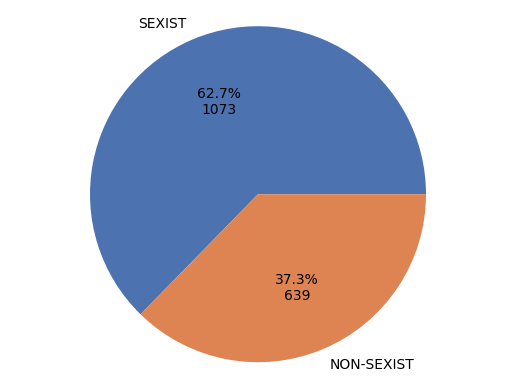
\includegraphics[height=0.4\textheight, width=\textwidth, keepaspectratio]{images/t4_es_hard_presentacion.png}%
            \vfill
            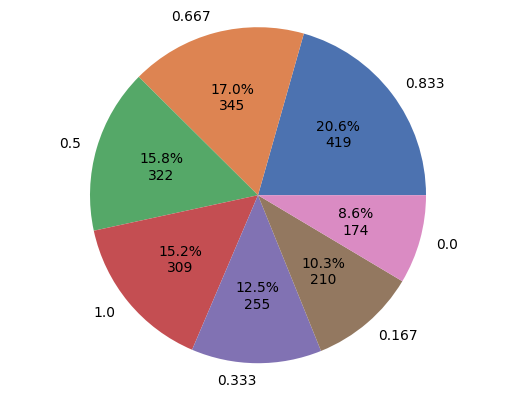
\includegraphics[height=0.4\textheight, width=\textwidth, keepaspectratio]{images/t4_es_soft_presentacion.png}%
        \end{column}

        \begin{column}{0.3\textwidth}
            \centering %Uncomment this line for horizontal centering 
            \textbf{Task 5}

            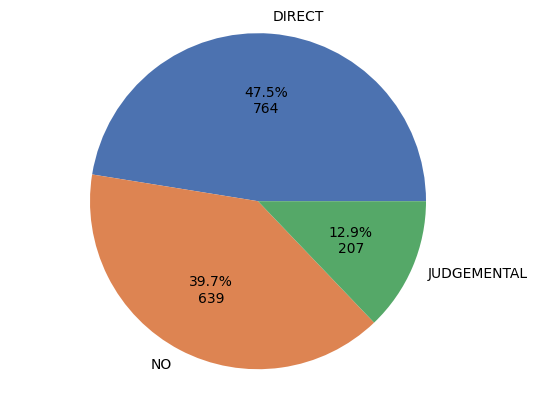
\includegraphics[height=0.4\textheight, width=\textwidth, keepaspectratio]{images/t5_es_hard_presentacion.png}%
            \vfill
            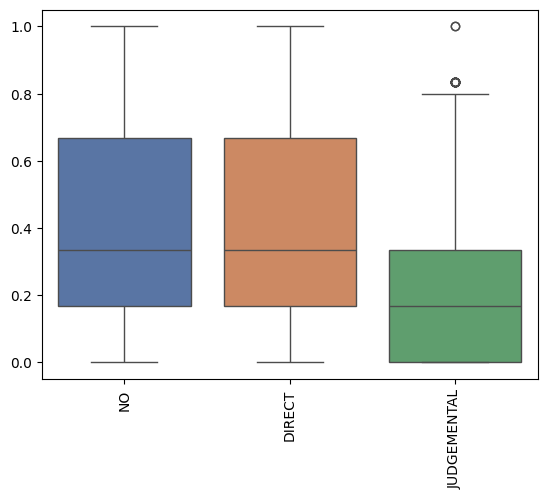
\includegraphics[height=0.4\textheight, width=\textwidth, keepaspectratio]{images/t5_es_soft_presentacion.png}%
        \end{column}

        \begin{column}{0.3\textwidth}
            \centering %Uncomment this line for horizontal centering
            \textbf{Task 6}

            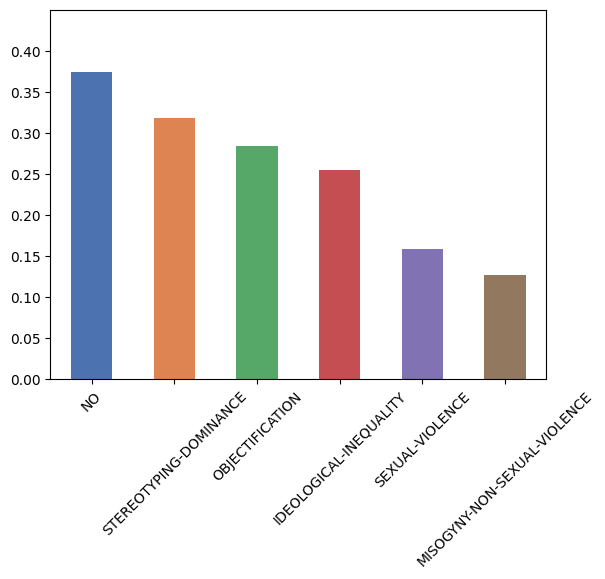
\includegraphics[height=0.4\textheight, width=\textwidth, keepaspectratio]{images/t6_es_hard_presentacion.png}%
            \vfill
            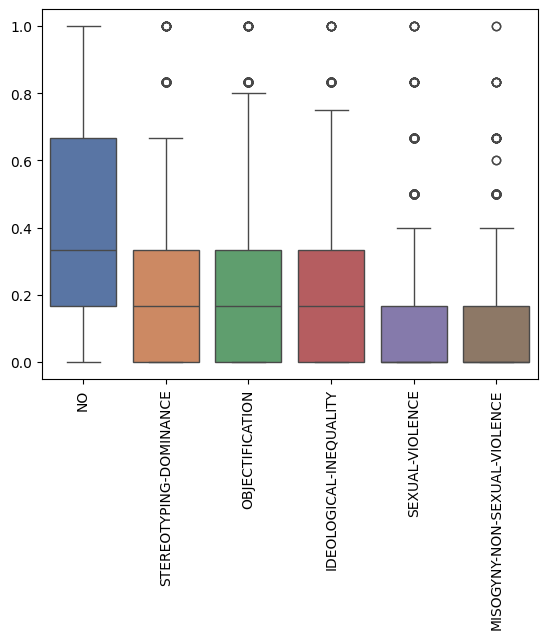
\includegraphics[height=0.4\textheight, width=\textwidth, keepaspectratio]{images/t6_es_soft_presentacion.png}%
        \end{column}
    \end{columns}
\end{frame}

\begin{frame}{Dataset (EN)}
    \begin{columns}[T]
        \begin{column}{0.3\textwidth}
            %\centering %Uncomment this line for horizontal centering 
            \centering
            \textbf{Task 4}

            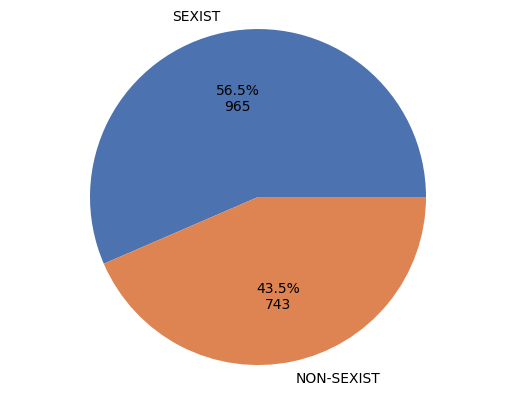
\includegraphics[height=0.4\textheight, width=\textwidth, keepaspectratio]{images/t4_en_hard_presentacion.png}%
            \vfill
            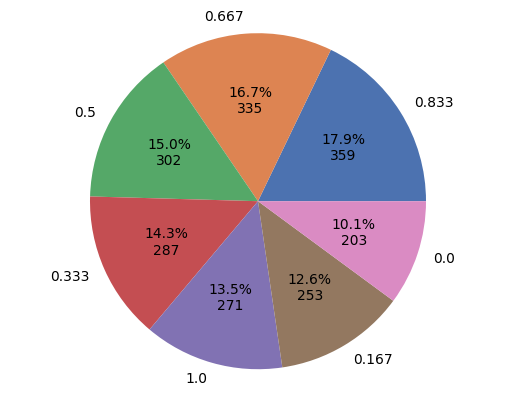
\includegraphics[height=0.4\textheight, width=\textwidth, keepaspectratio]{images/t4_en_soft_presentacion.png}%
        \end{column}

        \begin{column}{0.3\textwidth}
            \centering %Uncomment this line for horizontal centering 
            \textbf{Task 5}

            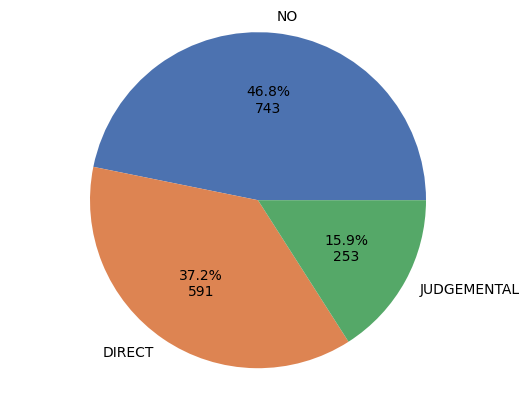
\includegraphics[height=0.4\textheight, width=\textwidth, keepaspectratio]{images/t5_en_hard_presentacion.png}%
            \vfill
            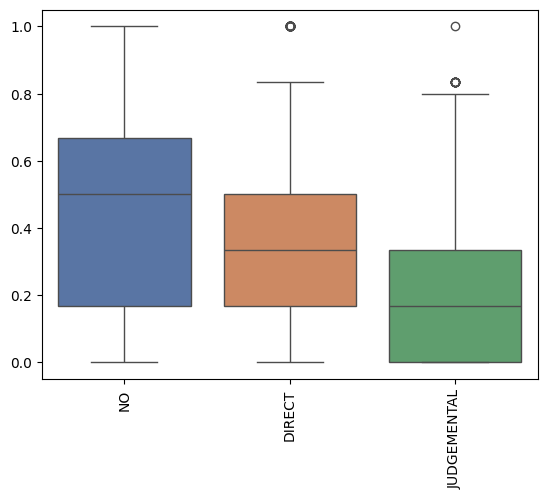
\includegraphics[height=0.4\textheight, width=\textwidth, keepaspectratio]{images/t5_en_soft_presentacion.png}%
        \end{column}

        \begin{column}{0.3\textwidth}
            \centering %Uncomment this line for horizontal centering
            \textbf{Task 6}

            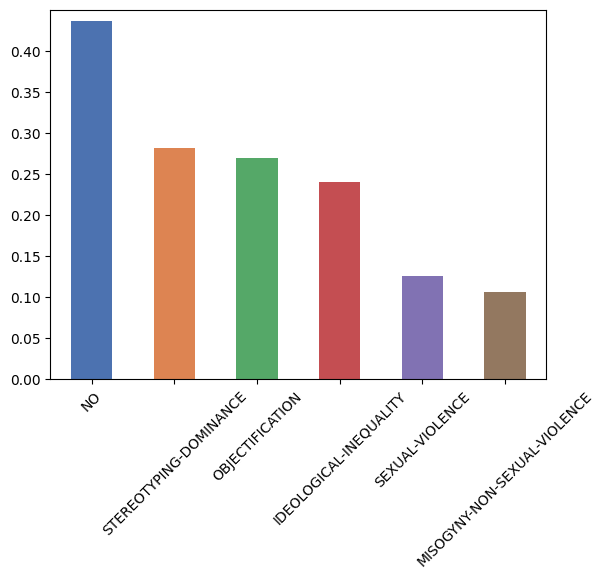
\includegraphics[height=0.4\textheight, width=\textwidth, keepaspectratio]{images/t6_en_hard_presentacion.png}%
            \vfill
            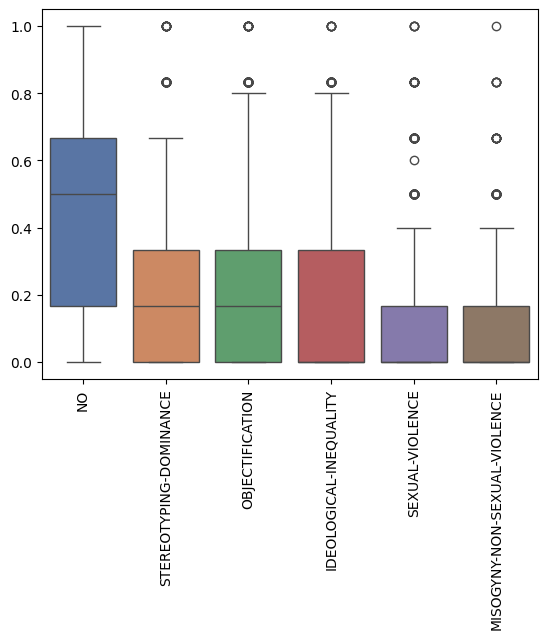
\includegraphics[height=0.4\textheight, width=\textwidth, keepaspectratio]{images/t6_en_soft_presentacion.png}%
        \end{column}
    \end{columns}
\end{frame}
%Propuesta del sistema
\begin{frame}{System proposals}

\begin{columns}
    \column{0.5\textwidth}
        \begin{itemize}
            \item Comparison of different modalities:
                \begin{itemize}
                    \item Unimodal architectures: \textit{Transformer encoder} (RoBERTa and ViT)
                    \item Multimodal architecture: \textit{Early fusion} by concatenating the [CLS] token
                \end{itemize}
            \item LeWiDi approaches:
                \begin{itemize}
                    \item Hard label
                    \item Soft label
                    \item \textbf{\textit{Why no multi-task approach?}}
                \end{itemize}
            \item One model for each language 
    \end{itemize}
    \column{0.5\textwidth}
    \centering
    \includesvg[width=0.8\textwidth]{images/unimodal.svg}
    \includesvg[width=0.45\textwidth]{images/early_fusion.svg}
\end{columns}
\end{frame}


\begin{frame}{Enhancing textual modality performance}
    \begin{columns}
        \column{0.5\textwidth}
        \centering 
        \begin{itemize}
            \item Textual preprocessing to remove noise (watermarks, emojis, URLS...)
            \item Avoid biases by masking \textit{identity term} 
            \item \textbf{Closing the visual and textual gap: meme descriptions (LLaVa)}
            \item \textbf{Data augmentation by incorporating tweets on the training dataset} \footnote{Available on text-only. Task 5 avoided.}
        \end{itemize}
        \column{0.5\textwidth}
        \centering
        \begin{figure}
            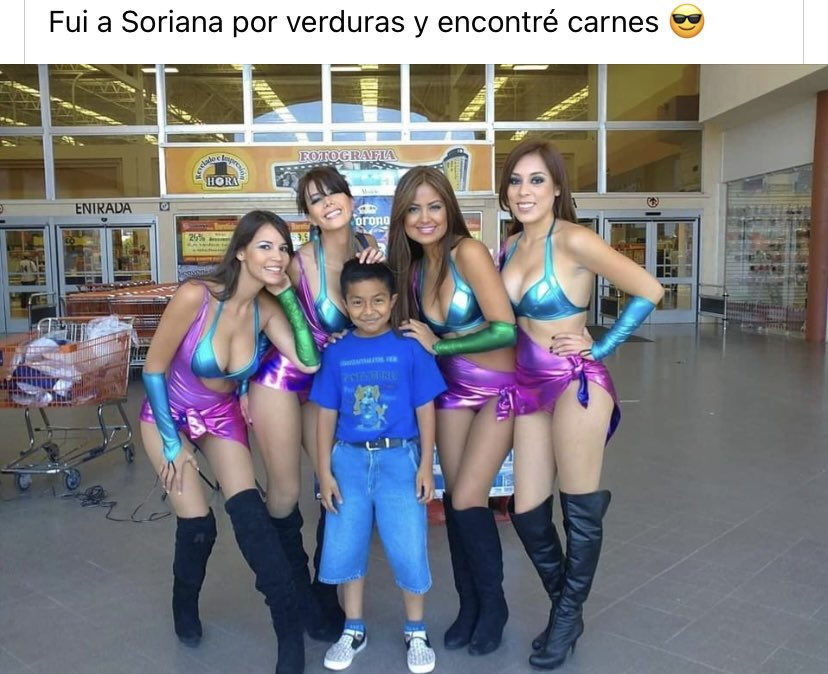
\includegraphics[width=\textwidth]{images/111702.jpeg}
            \caption{A group of women and a children pose for a photo.}
        \end{figure}
    \end{columns}

\end{frame}


%Resultados T4
\begin{frame}{Task 4: Sexism Identification in Memes}
\only<1>{
\begin{table}[]
\centering
\begin{adjustbox}{width=0.95\textwidth}
\begin{tabular}{|c|c|c|c|c|c|}
\hline
Architecture                                                                     & Label & Ranking     & ICM $\uparrow$ & ICM Norm $\uparrow$ & F1 - Sexist $\uparrow$ \\ \hline
\multirow{2}{*}{Text + CTXT}                                                    & Hard  & 14          & 0.087          & 0.544               & 0.729                  \\ \cline{2-6} 
                                                                                 & Soft  & 13          & 0.088          & 0.545               & 0.697                  \\ \hline
\multirow{2}{*}{\begin{tabular}[c]{@{}c@{}}Text + CTXT +\\ Tweets\end{tabular}} & Hard  & 29          & -0.093         & 0.453               & 0.684                  \\ \cline{2-6} 
                                                                                 & Soft  & 8           & 0.104          & 0.553               & 0.716                  \\ \hline
\multirow{2}{*}{Image}                                                           & Hard  & 43          & -0.312         & 0.341               & 0.677                  \\ \cline{2-6} 
                                                                                 & Soft  & 45          & -0.359         & 0.317               & 0.640                  \\ \hline
\multirow{2}{*}{Early}                                                           & Hard  & $4^\dagger$ & \textbf{0.166} & \textbf{0.584}      & \textbf{0.736}         \\ \cline{2-6} 
                                                                                 & Soft  & 34          & -0.165         & 0.416               & 0.652                  \\ \hline \hline
Gold Baseline                                                                    & -     & 0           & 0.983          & 1.000               & 1.000                  \\ \hline
Ganadores                                                                        & -     & 1           & 0.318          & 0.662               & 0.764                  \\ \hline
\end{tabular}%
\end{adjustbox}
\caption{Test results for the hard evaluation in task 4 of EXIST. In bold, our best results by metric. $\dagger$ denotes our best ranking.}
\label{tab:exist_t4_hard}
\end{table}
\footfullcite{Plaza2024OverviewOE}
}

\only<2>{
\begin{table}[]
\centering
\begin{adjustbox}{width=0.95\textwidth}

\begin{tabular}{|c|c|c|c|c|c|}
\hline
Architecture                                                                     & Label & Ranking     & ICM Soft $\uparrow$ & ICM Soft Norm $\uparrow$ & \textit{Cross Entropy} $\downarrow$ \\ \hline
\multirow{2}{*}{Text + CTXT}                                                    & Hard  & 2           & -0.201              & 0.468                    & 0.969                               \\ \cline{2-6} 
                                                                                 & Soft  & 25          & -0.679              & 0.391                    & 0.925                               \\ \hline
\multirow{2}{*}{\begin{tabular}[c]{@{}c@{}}Text + CTXT +\\ Tweets\end{tabular}} & Hard  & 17          & -0.546              & 0.412                    & 1.077                               \\ \cline{2-6} 
                                                                                 & Soft  & 11          & -0.430              & 0.431                    & \textbf{0.918}                      \\ \hline
\multirow{2}{*}{Image}                                                           & Hard  & 27          & -0.947              & 0.348                    & 1.033                               \\ \cline{2-6} 
                                                                                 & Soft  & 34          & -1.160              & 0.314                    & 1.015                               \\ \hline
\multirow{2}{*}{Early}                                                           & Hard  & $1^\dagger$ & \textbf{-0.118}     & \textbf{0.481}           & 1.081                               \\ \cline{2-6} 
                                                                                 & Soft  & 26          & -0.869              & 0.360                    & 0.980                               \\ \hline \hline
Gold Baseline                                                                    & -     & 0           & 3.111               & 1.000                    & 0.585                               \\ \hline
Ganadores                                                                        & -     & 1           & -0.293              & 0.453                    & 1.103                               \\ \hline
\end{tabular}%

\end{adjustbox}
\caption{Test results for the soft evaluation in task 5 of EXIST. In bold, our best results by metric. $\dagger$ denotes our best ranking.}
\label{tab:exist_task4_soft}
\end{table}
\footfullcite{Plaza2024OverviewOE}
}
\end{frame}

%Resultados T5
\begin{frame}{Task 5: Source Intention in Memes}

\only<1>{
\begin{table}[]
\centering
\begin{adjustbox}{width=0.95\textwidth}
    \begin{tabular}{|c|c|c|c|c|c|}
        \hline
        Architecture                  & Label & Ranking     & ICM $\uparrow$  & ICM Norm $\uparrow$ & F1 - Sexist $\uparrow$ \\ \hline
        \multirow{2}{*}{Text + CTXT} & Hard  & 6           & -0.272          & 0.406               & 0.382                  \\ \cline{2-6} 
                                      & Soft  & $1^\dagger$ & \textbf{-0.207} & \textbf{0.428}      & 0.400                  \\ \hline
        \multirow{2}{*}{Image}        & Hard  & 16          & -0.654          & 0.273               & 0.294                  \\ \cline{2-6} 
                                      & Soft  & 20          & -0.752          & 0.239               & 0.315                  \\ \hline
        \multirow{2}{*}{Early}        & Hard  & 13          & -0.360          & 0.375               & 0.377                  \\ \cline{2-6} 
                                      & Soft  & 2           & -0.237          & 0.418               & \textbf{0.411}         \\ \hline \hline
        Gold Baseline                 & -     & 0           & 1.438           & 1.000               & 1.000                  \\ \hline
        Ganadores                     & -     & 1           & -0.240          & 0.417               & 0.387                  \\ \hline
        \end{tabular}%
\end{adjustbox}
\caption{Test results for the hard evaluation in task 5 of EXIST. In bold, our best results by metric. $\dagger$ denotes our best ranking.}
\label{tab:exist_t5_hard}
\end{table}
\footfullcite{Plaza2024OverviewOE}
}

\only<2>{
\begin{table}[]
\centering
\begin{adjustbox}{width=\textwidth}
    \begin{tabular}{|c|c|c|c|c|c|}
        \hline
        Architecture                  & Label & Ranking     & ICM Soft $\uparrow$ & ICM Soft Norm $\uparrow$ & \textit{Cross Entropy} $\downarrow$ \\ \hline
        \multirow{2}{*}{Text + CTXT} & Hard  & $3^\dagger$ & \textbf{-1.323}     & \textbf{0.359}           & 1.602                               \\ \cline{2-6} 
                                      & Soft  & 8           & -1.620              & 0.328                    & 1.449                               \\ \hline
        \multirow{2}{*}{Image}        & Hard  & 10          & -1.969              & 0.291                    & 1.565                               \\ \cline{2-6} 
                                      & Soft  & 13          & -2.012              & 0.286                    & 1.512                               \\ \hline
        \multirow{2}{*}{Early}        & Hard  & 9           & -1.620              & 0.328                    & 1.520                               \\ \cline{2-6} 
                                      & Soft  & 5           & -1.377              & 0.354                    & \textbf{1.434}                      \\ \hline \hline
        Gold Baseline                 & -     & 0           & 4.702               & 1.000                    & 0.933                               \\ \hline
        Ganadores                     & -     & 1           & -1.245              & 0.368                    & 1.624                               \\ \hline
        \end{tabular}%
\end{adjustbox}
\caption{Test results for the soft evaluation in task 5 of EXIST. In bold, our best results by metric. $\dagger$ denotes our best ranking.}
\label{tab:exist_t5_soft}
\end{table}
\footfullcite{Plaza2024OverviewOE}
}

\end{frame}

%Resultados T6
\begin{frame}{Task 6: Sexism Categorization in Memes}
    \only<1>{
    \begin{table}[]
    \begin{adjustbox}{width=0.95\textwidth}
        \begin{tabular}{|c|c|c|c|c|c|}
            \hline
            Architecture                                                                     & Label & Ranking     & ICM $\uparrow$  & ICM Norm $\uparrow$ & F1 - Sexist $\uparrow$ \\ \hline
            \multirow{2}{*}{Text + CTXT}                                                    & Hard  & $2^\dagger$ & \textbf{-0.783} & \textbf{0.338}      & 0.402                  \\ \cline{2-6} 
                                                                                             & Soft  & 5           & -0.853          & 0.323               & 0.380                  \\ \hline
            \multirow{2}{*}{\begin{tabular}[c]{@{}c@{}}Text + CTXT +\\ Tweets\end{tabular}} & Hard  & 8           & -1.057          & 0.281               & 0.387                  \\ \cline{2-6} 
                                                                                             & Soft  & 3           & -0.810          & 0.332               & \textbf{0.434}         \\ \hline
            \multirow{2}{*}{Image}                                                           & Hard  & 20          & -1.647          & 0.158               & 0.222                  \\ \cline{2-6} 
                                                                                             & Soft  & 21          & -1.652          & 0.157               & 0.202                  \\ \hline
            \multirow{2}{*}{Early}                                                           & Hard  & 11          & -1.212          & 0.249               & 0.289                  \\ \cline{2-6} 
                                                                                             & Soft  & 12          & -1.270          & 0.237               & 0.316                  \\ \hline \hline
            Gold Baseline                                                                    & -     & 0           & 2.410           & 1.000               & 1.000                  \\ \hline
            Ganadores                                                                        & -     & 1           & -0.700          & 0.355               & 0.432                  \\ \hline
            \end{tabular}%
    \end{adjustbox}
    \caption{Test results of the hard evaluation in task 6 of EXIST. In bold, our best results by metric. $\dagger$ denotes our best ranking.}
    \label{tab:exist_t6_hard}
    \end{table}
    \footfullcite{Plaza2024OverviewOE}
    }
    \only<2>{
    \begin{table}[]
    \centering
    \begin{adjustbox}{width=0.95\textwidth}
        \begin{tabular}{|c|c|c|c|c|}
            \hline
            Architecture                                                                     & Label & Ranking     & ICM Soft $\uparrow$ & ICM Soft Norm $\uparrow$ \\ \hline
            \multirow{2}{*}{Text + CTXT}                                                    & Hard  & 9           & -5.737              & 0.196                    \\ \cline{2-5} 
                                                                                             & Soft  & 2           & -4.609              & 0.256                    \\ \hline
            \multirow{2}{*}{\begin{tabular}[c]{@{}c@{}}Text + CTXT +\\ Tweets\end{tabular}} & Hard  & 20          & -8.080              & 0.072                    \\ \cline{2-5} 
                                                                                             & Soft  & $1^\dagger$ & \textbf{-4.310}     & \textbf{0.272}           \\ \hline
            \multirow{2}{*}{Image}                                                           & Hard  & 11          & -6.411              & 0.160                    \\ \cline{2-5} 
                                                                                             & Soft  & 14          & -6.519              & 0.155                    \\ \hline
            \multirow{2}{*}{Early}                                                           & Hard  & 7           & -5.472              & 0.210                    \\ \cline{2-5} 
                                                                                             & Soft  & 8           & -5.550              & 0.206                    \\ \hline \hline
            Gold Baseline                                                                    & -     & 0           & 9.434               & 1.000                    \\ \hline
            Ganadores                                                                        & -     & 1           & -4.904              & 0.245                    \\ \hline
            \end{tabular}%
    \end{adjustbox}

    
    \caption{Test results of the soft evaluation in task 6 of EXIST. In bold, our best results by metric. $\dagger$ denotes our best ranking.}
    \label{tab:t6_exist_soft}
    \end{table}
    \footfullcite{Plaza2024OverviewOE}
    }
\end{frame}

%Conclusiones
\section{Conclusions and future work}


\begin{frame}{Conclusions}
\begin{itemize}
    \item \textbf{RQ1}:
    \begin{itemize}
        \item Competitive results
        \item LeWiDi models achieve better results
        \item LeWiDi models generalize better
        \item Insights into the flaws of the multi-task approach
        \item Context and data augmentation
        \item Fine-tuning strategy
        \item Difficulty of the implicit detection task 
    \end{itemize} 
    \item \textbf{RQ2}:
    \begin{itemize}
        \item Competitive results, even surpassing SOTA results
        \item Text $\textgreater$ Image
        \item Importance of text description
        \item LeWiDi models offer better generalization
        \item Image-text relation in memes is very complex.
    \end{itemize}
\end{itemize}   
\end{frame}

\begin{frame}{Future work (and some tips for EXIST 2025...)}
    \begin{itemize}
        \item On BERT fine-tuning:
        \begin{itemize}
            \item Intermediate tasks for boosting performance
            \item Fine-tuned models on HF from similar tasks
            \item Re-init BERT layers
        \end{itemize}
        \item Stereotype on multimodal detection: 
        \begin{itemize}
            \item \textbf{External features are important, but so are the selected models}
            \item Image/video description: \textbf{Qwen2.5 VL, GPT-like, SmolVLM2, Llama3.2 11B, Gemma 3}
            \item Image features: \textbf{YOLO, Faster R-CNN, EfficientNet}
            \item Improve text-image alignment
        \end{itemize} 
        \item LLM's
        \begin{itemize}
            \item Data augmentation
            \item Few-shot
            \item Provide explanations
        \end{itemize}
        \item Alternatives approaches for LeWiDi:
        \begin{itemize}
            \item \textbf{Multi-task} with \textbf{hard and soft labels} 
            \item Perspectivist approach in EXIST with clustering and demographic information
        \end{itemize}
    \end{itemize}
    
\end{frame}



\appendix
\begin{frame}{}
    \begin{center}
        \Huge Thanks for your attention!
        
        \Huge Any questions?
    \end{center}
    \adjustbox{valign=c, width=3cm}{
\includegraphics{images/logoprhlt_mobil.png}}%
    \hfill
    \adjustbox{valign=c, width=1.5cm}{\includesvg{images/marca_UPV_secundaria_negro.svg}}%
\end{frame}

\begin{frame}{ICM}
    \only<1>{
        \begin{itemize}
            \item Formula:
            $$
            ICM(A, B)= 2IC(A) + 2IC(B) - 3IC(A \cup B)
            $$
            \item \textit{Information Content} of one category:
            \begin{align*}
                IC(c_i) &= -\log_2(P(c_i)) \\
                &\simeq -\log_{2} \left(\frac{|\bigcup_{c' \in \{c\} \cup \text{Desc}(c')} \mathcal{I}_{c'}|}{|\bigcup_{c' \in \mathcal{C}} \mathcal{I}_{c'}|}\right)
            \end{align*}
            \item IC of a set of categories:
            \begin{align*}
                IC(\{c_i\} \cup \{c_j\}) &= IC(c_i) + IC(c_j) - IC(\{c_i\} \cap \{c_j\}) \\
                &= IC(c_i) + IC(c_j) - IC(\text{lso}(c_i, c_j))
            \end{align*}
        \end{itemize}
    }

    \only<2>{
        \begin{columns}[T]
            \column{0.3\textwidth}
            \begin{itemize}
                \item Email:
                \begin{itemize}
                    \item Spam (S)
                    \begin{itemize}
                        \item Scam (SC)
                        \item Travels (TR)
                    \end{itemize}
                    \item NoSpam (NS)
                \end{itemize}
            \end{itemize}

            \column{0.5\textwidth}
            \begin{table}[]
                \centering
                \begin{tabular}{|c|c|c|}
                    \hline
                    \textbf{ID} & \textbf{TRUTH} & \textbf{PRED} \\ \hline
                    1 & NS & NS \\ \hline
                    2 & TR, SC & TR \\ \hline
                    3 & SC & NS \\ \hline
                    4 & NS & NS \\ \hline
                    5 & TR & SC \\ \hline
                    6 & NS & NS \\ \hline
                    7 & NS & NS \\ \hline
                \end{tabular}
            \end{table}
        \end{columns}
    }

    \only<3>{
        \begin{itemize}
            \item A prioris:
            \begin{align*}
                P(\text{NS}) &= \frac{4}{7} \approx 0.571 \\
                P(\text{S}) &= \frac{3}{7} \approx 0.429 \\
                P(\text{SC}) &= P(\text{TR}) = \frac{2}{7} \approx 0.2857 \\
            \end{align*}
            \item IC:
            \begin{align*}
                IC(\text{NS}) &= - \log_2 P(\text{NS}) = - \log_2 0.571 \approx 0.80 \\
                IC(\text{S}) &= - \log_2 P(\text{S}) = - \log_2 0.429 \approx 1.22 \\
                IC(\text{SC}) &= IC(\text{TR}) = - \log_2 0.2857 \approx 1.80
            \end{align*}
        \end{itemize}
    }

    \only<4>{
        \begin{itemize}
            \item ID 1, 4, 6, 7:
            \begin{align*}
                ICM(\text{NS}, \text{NS}) &= 2IC(\text{NS}) + 2IC(\text{NS}) - 3IC( \{\text{NS}\} \cup \{\text{NS}\}) \\
                &= 4IC(\text{NS}) - 3IC( \text{NS}) = IC(\text{NS}) \\
                &= 0.80
            \end{align*}
            \item ID 2:
            \begin{align*}
                IC(\{\text{TR, SC}\}, \{\text{TR}\}) &= 2IC(\{\text{TR, SC}\}) + 2IC(\{\text{TR}\}) - 3IC(\{\text{TR, SC}\}) \\
                &= 2IC(\{\text{TR}\}) - IC(\{\text{TR, SC}\})\\
                &= 2 \cdot 1.8 - 2.38 = 1.22
            \end{align*}
            \begin{align*}
                IC(\{\text{TR, SC}\}) &= IC(\text{TR}) + IC(\text{SC}) - IC(\text{lso}(\text{TR}, \text{SC})) \\
                &= IC(\text{TR}) + IC(\text{SC}) - IC(\text{S}) \\
                &= 1.80 + 1.80 - 1.22 = 2.38
            \end{align*}
        \end{itemize}
    }

    \only<5>{
        \begin{itemize}
            \item ID 3:
            \begin{align*}
                ICM(\text{SC}, \text{NS}) &= 2IC(\text{SC}) + 2IC(\text{NS}) - 3IC(\{\text{SC}\} \cup \{\text{NS}\}) \\
                &= 2\cdot1.8 + 2\cdot0.8 - 3\cdot2.6 = -2.6
            \end{align*}
            \begin{align*}
                IC(\{\text{SC}, \text{NS}\}) &= IC(\text{SC}) + IC(\text{NS}) - IC(\text{lso}(\text{SC}, \text{NS})) \\
                &= 1.80 + 0.80 - 0 = 2.6
            \end{align*}
            \item ID 5:
            \begin{align*}
                ICM(\text{SC}, \text{TR}) &= 2IC(\text{SC}) + 2IC(\text{TR}) - 3IC(\{\text{SC}, \text{TR}\}) \\
                &= 2\cdot1.80 + 2\cdot1.80 - 3\cdot2.38 = 0.06
            \end{align*}
        \end{itemize}
    }
    \only<6>{
        Average ICM:
        \begin{align*}
            \frac{4 \cdot 0.8 + 1.22 - 2.6 + 0.06}{7} \approx 0.2685
        \end{align*}
    }
\end{frame}

\end{document}
